%%%%%%%%%%%%%%%%%%%%%%%%%%%%%%%%%%%%%%%%%%%%%%%%%%%%%%%%%%%%
%%  This Beamer template was created by Cameron Bracken.
%%  Anyone can freely use or modify it for any purpose
%%  without attribution.
%%
%%  Last Modified: January 9, 2009
%%

\documentclass[xcolor=x11names,compress]{beamer}
\usepackage[utf8]{inputenc} 
\usepackage[T1]{fontenc}
\usepackage{cmbright}

%% General document %%%%%%%%%%%%%%%%%%%%%%%%%%%%%%%%%%
\usepackage{graphicx}
\usepackage{tikz}

\usepackage[style=authoryear]{biblatex}
\usetikzlibrary{decorations.fractals}
%%%%%%%%%%%%%%%%%%%%%%%%%%%%%%%%%%%%%%%%%%%%%%%%%%%%%%


%% Beamer Layout %%%%%%%%%%%%%%%%%%%%%%%%%%%%%%%%%%
\useoutertheme[subsection=false,shadow]{miniframes}
\setbeamerfont{title like}{shape=\scshape}
\setbeamerfont{frametitle}{shape=\scshape}

\setbeamercolor*{lower separation line head}{bg=DeepSkyBlue4} 
\setbeamercolor*{normal text}{fg=black,bg=white} 
\setbeamercolor*{alerted text}{fg=red} 
\setbeamercolor*{example text}{fg=black} 
\setbeamercolor*{structure}{fg=black} 

 \usenavigationsymbolstemplate{}
\setbeamercolor*{palette tertiary}{fg=black,bg=black!10} 
\setbeamercolor*{palette quaternary}{fg=black,bg=black!10} 

\renewcommand{\(}{\begin{columns}}
\renewcommand{\)}{\end{columns}}
\newcommand{\<}[1]{\begin{column}{#1}}
\renewcommand{\>}{\end{column}}
%%%%%%%%%%%%%%%%%%%%%%%%%%%%%%%%%%%%%%%%%%%%%%%%%%
\useoutertheme{infolines} % authors, etc.
%%%%%%%%%%%%%%%%%%%%%%%%%%%%%%%%%%%%%%%%%%%%%%%%%%

\bibliography{presentation.bib}

\DeclareGraphicsExtensions{.pdf,.png,.jpg, .eps}

\usepackage{color, colortbl}  
\definecolor{LightCyan}{rgb}{0.88,0.8,1}
\begin{document}


\begin{frame}{}
\title[Neocortex]{A network model of the neocortex}
\author{
Friedrich Schüßler}
\date{\today}
\titlepage

\centering 
Supervisor: Prof. Stefan Rotter
\end{frame}

\begin{frame}{Table of contents}
    \tableofcontents
\end{frame}

\AtBeginSection[]{
\begin{frame}{Table of contents}
    \tableofcontents[currentsection]
\end{frame}
}


\section{Intro}
\begin{frame}[t]{Introduction}
Here could be a figure //
Subtitle to figure
\end{frame}

\section{Section 1}
\begin{frame}[t]{Network model}
\begin{figure}[htpb]
    \centering
    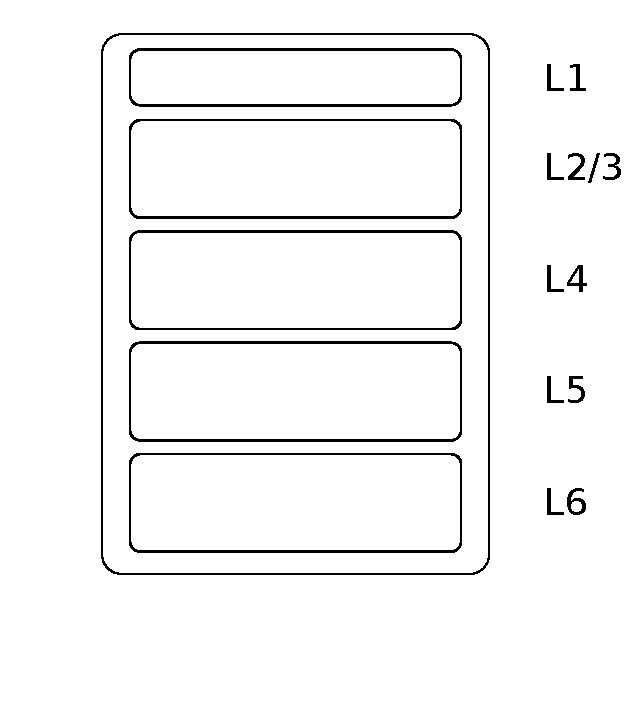
\includegraphics[width=0.5\linewidth]{../figures/microcircuit_model_pre}
\label{fig:setup_1}
\end{figure}
\end{frame}

\begin{frame}[t]{Network model}
\begin{figure}[htpb]
    \centering
    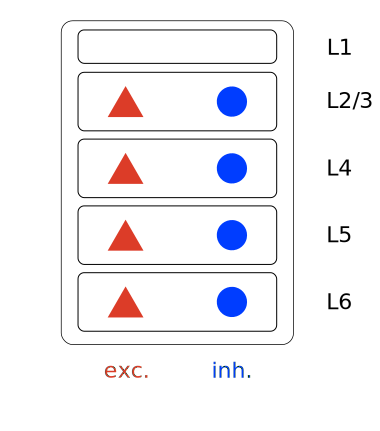
\includegraphics[width=0.5\linewidth]{../figures/microcircuit_model_pre0}
\label{fig:setup_1}
\end{figure}
\end{frame}

\begin{frame}[t]{Network model}
\begin{figure}[htpb]
    \centering
    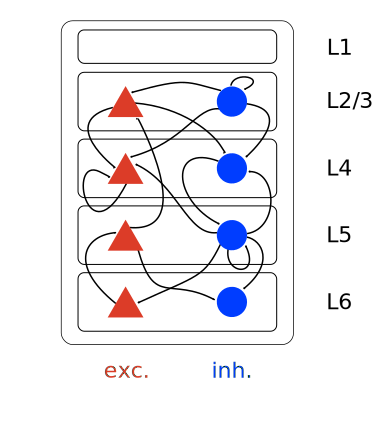
\includegraphics[width=0.5\linewidth]{../figures/microcircuit_model_pre1}
\label{fig:setup_1}
\end{figure}
\end{frame}

\begin{frame}[t]{Network model}
\begin{figure}[htpb]
    \centering
    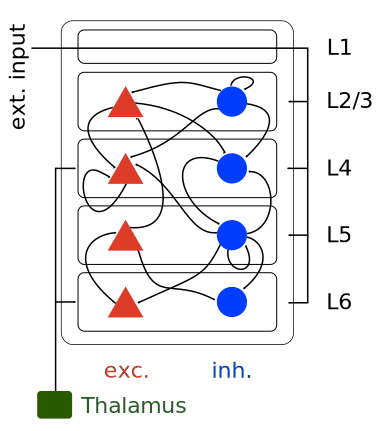
\includegraphics[width=0.5\linewidth]{../figures/microcircuit_model_full}
\label{fig:setup_1}
\end{figure}
\end{frame}

\begin{frame}[t]{Network parameters}
\begin{table}[htpb]
    \centering
    \label{tab:network_parameters}
    \begin{tabular}{l l}
        \rowcolor{LightCyan} Parameter specification & \\
        \cellcolor{LightCyan} Total population size & $\approx 80,000$\\
        \cellcolor{LightCyan} Total synapse number  & $\approx 0.3 * 10^9$\\
        \cellcolor{LightCyan} Neuron model& leaky integrate-and-fire\\
        \cellcolor{LightCyan} Rel. inh. synaptic strength & $g = -4.0$\\
    \end{tabular}
\end{table}
\end{frame}


\section{Section 2}
\begin{frame}[t]{Formulas}
    Klein-Nishina Formula
\begin{equation}
    \frac{\text{d} \sigma_\text{C}}{\text{d} E_{e, \text{kin}}} 
    = \frac{\alpha^2 \lambda_e^2}{16 \pi^3 m_e c^2}  \frac{1}{a^2}\left(
        \frac{b^2}{a^2(a - b)^2} + \frac{(b - 1)^2 - 1}{a (a - b)} \right) 
    \label{eq:dode}
\end{equation}
with $a := E_\gamma / m_ec^2$ \\ 
and $b := E_{e, \text{kin}} / m_ec^2$ 
\end{frame}

\begin{frame}[t]{Table}
\begin{table}[htpb]
    \centering
    \label{tab:mono_calibration}
    \begin{tabular}{l l r c c}
        \rowcolor{LightCyan} Sample & Peak/Edge & $E$ / keV& NaI / Channel & PVC / Channel \\
        \cellcolor{LightCyan}$^{137}$Cs & Photo & 662 & $8040.59 \pm 0.03$ &  \\
        \cellcolor{LightCyan} & Compton& 477& $5720 \pm 4$ &  $178.9 \pm 0.3$  \\
        \cellcolor{LightCyan} & Backscatter& 183&  $2510 \pm 12$ &  \\
        \cellcolor{LightCyan}$^{22}$Na & Photo& 511& $6347 \pm 3$&  \\
        \cellcolor{LightCyan} & Compton& 341& $4000 \pm 2000$& $108 \pm 2$  \\
        \cellcolor{LightCyan} & Photo& 1277& $14180 \pm 20 $& \\
        \cellcolor{LightCyan} & Compton& 1064& $12000 \pm 4000$& $414 \pm 4$ \\
    \end{tabular}
\end{table}
\end{frame}


\section{Appendix}
\label{sec:appendix}
\begin{frame}[t]{Figure}
 \begin{figure}[htpb]
    \centering
    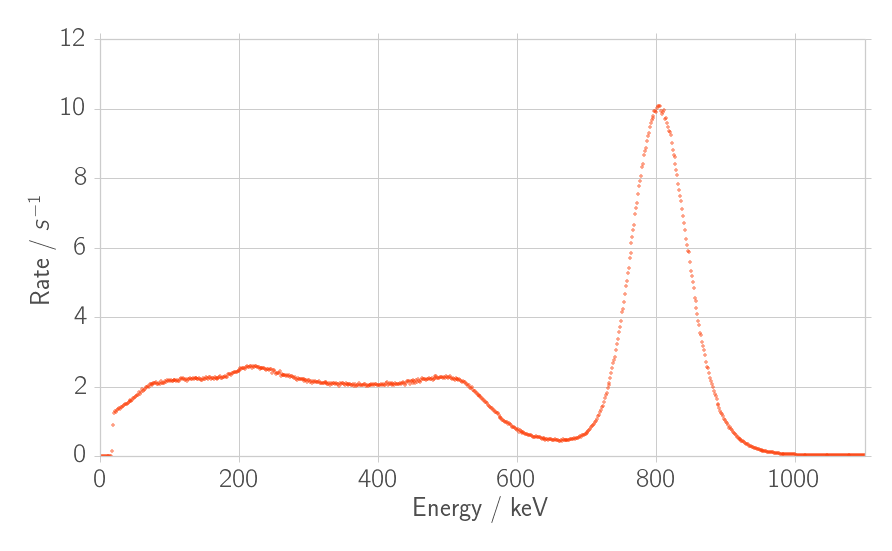
\includegraphics[width=1.0\linewidth]{../figures/na_total_incident}
    \label{fig:histo_na_137cs}
\end{figure}
\end{frame}


\end{document}
